\documentclass[11pt]{article}
\usepackage[T1]{fontenc}
\usepackage{lmodern,amsmath,booktabs,graphicx}
\usepackage[margin=1in]{geometry}
\usepackage[colorlinks=true,linkcolor=blue,citecolor=blue,urlcolor=blue]{hyperref}
\hypersetup{pdfauthor={Qianghao Wu},pdftitle={An inconclusive score of the 2017 Earth-rotation forecast of more global M>=7 earthquakes}}
\title{An inconclusive score of the 2017 Earth-rotation forecast\\ of more global $M\ge 7$ earthquakes}
\author{Qianghao Wu}
\date{November 25, 2026}
\begin{document}
\maketitle
\begin{abstract}
In 2017, Bilham and Bendick forecast that a slowing of Earth's rotation that began in 2011 would bring a period of at least five years with more global earthquakes of magnitude 7 or more. Their abstract gives a 25--30\% increase in such periods. We pre-registered a test of the forecast against the USGS ComCat catalog, and we disclose the counts that were seen before the protocol. ComCat lists 66 $M\ge7$ events in 2018--2022, or 13.2 per year. The 1900--2017 mean is 12.68 per year, so the observed rate is 1.04 times this baseline (95\% interval 0.78--1.39). Under a negative binomial model of annual counts, the +25\% level is not rejected ($p = 0.115$), and no increase above the baseline is shown ($p = 0.40$). The pre-registered verdict is inconclusive: one five-year window cannot separate no increase from an increase of 25\%. Under this rule, 61 events or fewer would have refuted the forecast, and 80 or more would have supported it. A held-out test of the five-year lag between rotation slowing and seismicity, on 2018--2025, gives a rate ratio of 0.98 (permutation $p = 0.61$). This test has a power of only 17\% for a 25\% effect, so it gives little information. In 1900--2017, the same lag statistic is largest at lags of 6--8 years (rate ratio about 1.1). Over all ten lags, this maximum is at the 97th percentile of a circular-shift null for the raw catalog and at the 86th percentile for a declustered catalog. These are tests of association in count data.

This work has not yet been reviewed by experts. The computations, the code and the text were produced by AI models (from Anthropic and OpenAI), working under the author's direction.
\end{abstract}
\medskip
\noindent\textit{Keywords:} earthquake forecasting, length of day, Earth rotation, global seismicity, pre-registration, forecast evaluation

\section{Introduction}
Bendick and Bilham reported that global earthquakes of magnitude 7 or more cluster in time and that their annual number varies with a period of about 32 years~\cite{bb2017,voosen2017}. At the Annual Meeting of the Geological Society of America in October 2017, Bilham and Bendick~\cite{gsa2017} linked this variation to changes in the length of day (LOD). Their abstract says:
\begin{quote}
``On five occasions in the past century a 25-30\% increase in annual numbers of Mw$\ge$7 earthquakes has coincided with a slowing in the mean rotation velocity of the Earth [\dots] The correlation between Earth's angular deceleration (d[LoD]/dt) and global seismic productivity is yet more striking, and can be shown to precede seismicity by 5-6 years [\dots] The year 2017 marks six years following a deceleration episode that commenced in 2011, suggesting that the world has now entered a period of enhanced global seismic productivity with a duration of at least five years.''
\end{quote}
The same abstract says that the delayed productivity is ``most pronounced at equatorial latitudes 10\textdegree N-30\textdegree S''. Science reported the talk~\cite{voosen2017}: ``Beginning next year, Earth should expect five more major earthquakes a year than average---between 17 to 20 quakes''. In the same article, James Dolan said: ``we're going to know in 5 years.''

The five years are now over. We give a pre-registered score of the forecast for 2018--2022. We also test the five-year lag on the eight years 2018--2025, which were not available in 2017.

\begin{quote}
\textbf{ComCat has 66 $M\ge7$ events in 2018--2022, 1.04 times the 1900--2017 rate. The data reject neither ``no increase'' nor ``+25\%''. The pre-registered verdict is inconclusive.}
\end{quote}

\subsection*{Earlier work}
Bendick and Bilham~\cite{bb2017} used a catalog that they describe as complete for $M_w \ge 7.1$ in 1900--2017. Bilham, Szeliga, Mencin and Bendick~\cite{bilham2022} moved to a forecast for the Caribbean to 2030. Their Fig.~1B gives a global lag statistic for 1900--2017 with a binary deceleration mask, against a random-catalog level of $51.7 \pm 1.3\%$. They note that some catalogs show a correlation that is significantly above random and that others do not. They do not score the 2017 global forecast. Bilham and Ghobadi-Far~\cite{bilham2025} propose a mechanism (Polflucht modulation of Coulomb failure). We did not read this four-page proceeding, because it is behind a paywall. Shearer and Stark~\cite{shearer2012} found that the declustered global catalog of $M\ge7$ events is consistent with a Poisson process. Jenkins, Biggs, Rust and Rougier~\cite{jenkins2021} compared decadal rates of earthquakes and volcanic eruptions. Dumont and colleagues~\cite{dumont2025} decomposed global $M\ge6$ counts with singular spectrum analysis and compared them with LOD and sea level. Doglioni~\cite{doglioni2026} found no coherence between LOD and global counts at the 18.6-year lunar nodal period, but reported a modulation of seismic moment release at that period. None of these works scores the 2017 forecast. Our search (Semantic Scholar and OpenAlex citations of~\cite{bb2017}, arXiv, OpenAlex, Zenodo, GitHub and web searches, November 2026) found no published score of it. One proceeding~\cite{bilham2025} was not read, so this statement has that limit.

\section{Data}
\paragraph{Earthquakes.} We use the USGS Comprehensive Catalog (ComCat)~\cite{comcat}: all events of type \texttt{earthquake} with preferred magnitude $\ge 7.0$, worldwide, all depths, from 1900-01-01 to 2025-12-31 UTC. The query of 2026-11-25 returned 1607 events. Years are UTC calendar years of the origin time. The magnitude is the ComCat preferred magnitude, which mixes magnitude types for early events.

\paragraph{Earth rotation.} The deceleration mask uses the EOP C02 series of the Paris Observatory~\cite{c02}, which gives LOD at 100-day steps from 1830. Before 1955 it is based on Jordi, Morrison and Rosen~\cite{jordi1994}. We interpolate linearly to daily values and take calendar-year means. The mask is $M(y) = 1$ if the mean LOD of year $y$ is larger than that of year $y-1$ (the Earth slowed down during year $y$), else $M(y)=0$. In C02 the annual LOD increases in each year 2011--2016 and decreases in each year 2017--2022. This agrees with the deceleration episode from 2011 that the source names. Of the years 1900--2017, 48\% are deceleration years. As a cross-check, the annual means of C02 and of the IERS EOP 20 C04 series~\cite{c04} have a correlation of 0.9991 in 1962--2024.

\section{Pre-registered tests}
We committed the protocol (included in the result folder as \texttt{PROTOCOL.md}) on 2026-11-25 at 18:04 CET, before the catalog was downloaded in that session. The commit time is the evidence. The commit order cannot prove that no catalog query happened before. The protocol discloses what was known before: informal annual counts for 2018--2021 (17, 10, 9, 19) and an unchecked count of 66 events for 2018--2022. So the direction of the main result was foreseeable. The decision rules do not depend on these numbers, and the power of each test is reported.

\paragraph{P1: the five-year forecast.} The baseline $\lambda_0$ is the mean annual count in 1900--2017. A negative binomial (NB) distribution is fitted to the 118 annual counts by the method of moments ($\mathrm{var} = \mu + \mu^2/k$). A five-year sum with annual rate $\lambda$ is NB with mean $5\lambda$ and size $5k$ (independent years). With $N$ the count in 2018--2022:
\[
p_{\text{refute}} = P(X \le N),\ X \sim \mathrm{NB}(5 \cdot 1.25\,\lambda_0,\ 5k); \qquad
p_{\text{support}} = P(X \ge N),\ X \sim \mathrm{NB}(5\lambda_0,\ 5k).
\]
The verdict is REFUTED if $p_{\text{refute}} < 0.05$, SUPPORTED if $p_{\text{support}} < 0.05$, and INCONCLUSIVE otherwise. The forecast level $1.25\,\lambda_0$ is the lower end of the stated 25--30\%. Eight secondary analyses (the seven variants in Table~1 and a comparison with 2013--2017) and two controls (placebo windows and known-answer injection) were fixed in advance. They do not change the verdict.

\paragraph{P2: held-out lag test.} For each year $y$ in 2018--2025, the year is ``predicted enhanced'' if $M(y-5)=1$. The statistic is the difference of the mean annual counts in predicted-enhanced years and in the other years. The $p$-value is an exact one-sided permutation test over all assignments of the same number of labels to the eight years. The verdict is SUPPORTED if $p < 0.05$, else NOT SUPPORTED. Lag 6, a declustered catalog and $M\ge7.1$ are secondary.

\paragraph{P3: in-sample lag curve, 1900--2017.} For lags $L = 0, \dots, 9$ we compute the share of events in years with $M(y-L)=1$ and the rate ratio. The null distributions are circular shifts of the mask by 10 to 108 years (99 shifts) and 10\,000 random catalogs with uniform years. P3 is descriptive and has no verdict.

\paragraph{Declustering.} We apply Gardner--Knopoff windows~\cite{gk1974} within the $M\ge7$ set, with the usual fit $d = 10^{0.1238M+0.983}$\,km and $t = 10^{0.032M+2.7389}$\,days~\cite{vanstiphout2012}. Events are processed by decreasing magnitude. This leaves 1395 of 1607 events.

\paragraph{A deviation, found after the results.} The protocol states 10\,000 simulations for the P2 power. The solve-stage code used 2000 simulations (power 0.172, false-positive rate 0.028). The released code also runs the pre-registered 10\,000 simulations, with a separate random generator so that no other number changes. They give a power of 0.170 and a false-positive rate of 0.034. We report the 10\,000-simulation values. A dated addendum to the protocol records this change. Some values in this paper are additions that the protocol does not list: the decision thresholds in $N$, $p_{\text{refute}}$ for other forecast levels, and the P2 test with a mask from C04. We label them as additions.

\section{Results}
\begin{figure}[t]
\centering
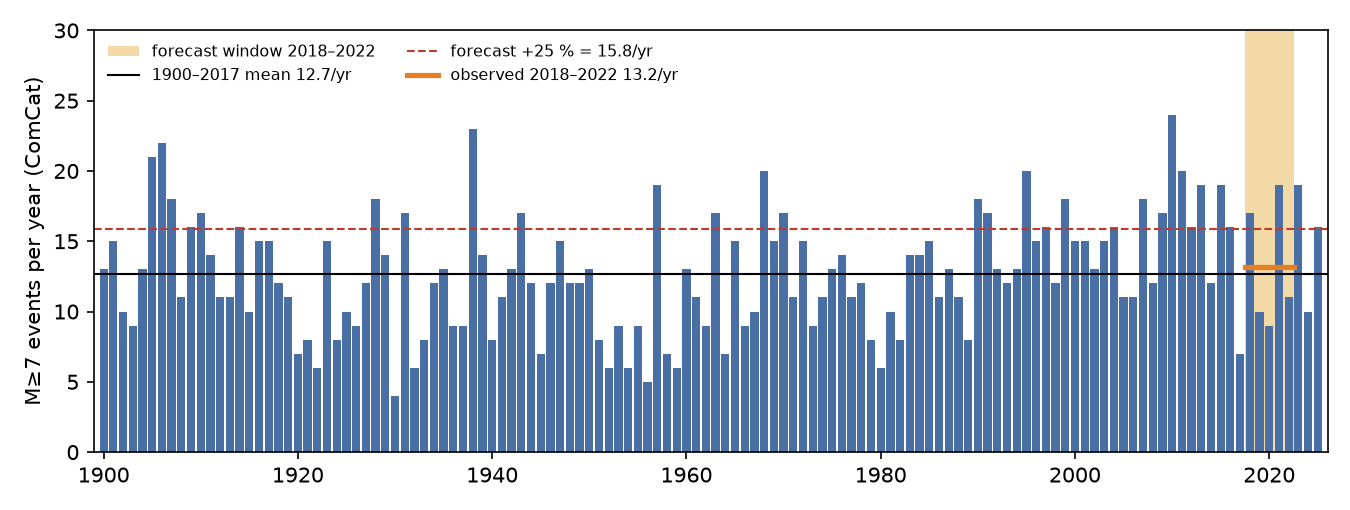
\includegraphics[width=\textwidth]{figures/fig1_counts.png}
\caption{Annual number of $M\ge7$ events in ComCat, 1900--2025. Black line: 1900--2017 mean (12.7 per year). Red dashed line: the forecast level $1.25\,\lambda_0$ (15.8 per year). Orange line: the observed 2018--2022 mean (13.2 per year).}
\end{figure}

\subsection{P1: the 2018--2022 window is inconclusive}
The baseline has 1496 events in 1900--2017: $\lambda_0 = 12.68$ per year, annual variance 17.35, NB size $k = 34.4$. The annual counts in 2018--2022 are 17, 10, 9, 19 and 11, so $N = 66$ (13.2 per year). The rate ratio is $1.04$, with a 95\% interval of 0.78--1.39. This interval contains both 1.00 and the forecast range 1.25--1.30. The p-values are $p_{\text{refute}} = 0.115$ and $p_{\text{support}} = 0.399$. The verdict is \textbf{INCONCLUSIVE}. The observed rate is near the baseline. The data cannot separate ``no increase'' from ``+25\%''.

Under this rule, $N \le 61$ would have given REFUTED and $N \ge 80$ would have given SUPPORTED (addition). The observed 66 is between these limits.

\paragraph{The forecast level is a reading of the source.} The abstract does not state the reference rate for the 25--30\%. Our $\lambda_0$ is the mean of all years 1900--2017, and this mean includes the enhanced periods. So $1.25\,\lambda_0$ is a high reading of the forecast. A lower reading is harder to refute. As an addition, $p_{\text{refute}}$ is 0.38 for a level of $1.10\,\lambda_0$, 0.31 for $1.13\,\lambda_0$, 0.18 for $1.20\,\lambda_0$ and 0.070 for $1.30\,\lambda_0$. Only levels of about $1.34\,\lambda_0$ or more give $p_{\text{refute}} < 0.05$. So no level in the stated 25--30\% changes the verdict.

\begin{table}[t]
\centering\footnotesize
\begin{tabular}{lrrrrrl}
\toprule
Variant & $N$ & Baseline/yr & Ratio & $p_{\text{refute}}$ & $p_{\text{support}}$ & Rule output\\
\midrule
Primary & 66 & 12.68 & 1.04 & 0.115 & 0.399 & inconclusive\\
Poisson instead of NB & 66 & 12.68 & 1.04 & 0.073 & 0.388 & inconclusive\\
$M\ge7.1$ & 51 & 9.92 & 1.03 & 0.124 & 0.443 & inconclusive\\
Declustered & 59 & 11.02 & 1.07 & 0.153 & 0.327 & inconclusive\\
Baseline 1973--2017 & 66 & 13.73 & 0.96 & 0.019 & 0.637 & below 0.05\\
Window 2017--2021 & 62 & 12.68 & 0.98 & 0.054 & 0.569 & inconclusive\\
Level 17 per year (press figure) & 66 & 12.68 & 1.04 & 0.045 & 0.399 & below 0.05\\
Sliding 5-year sums, 1900--2017 & 66 & -- & -- & 0.21 & 0.42 & inconclusive\\
\bottomrule
\end{tabular}
\caption{P1 and its pre-registered secondary analyses. Only the first row decides the verdict. ``Below 0.05'' means that $p_{\text{refute}} < 0.05$ in that variant. The sliding sums row gives the share of the 114 historical five-year sums $S$ (mean 63.4, SD 12.4) with $1.25\,S \le 66$ and with $S \ge 66$.}
\end{table}

\paragraph{Secondary analyses (Table 1).} Five of the seven variants give an inconclusive output. Two give $p_{\text{refute}} < 0.05$. We do not read either one as a refutation. First, the 1973--2017 baseline is 13.73 per year, higher than the 1900--1972 rate of 12.0 per year. Part of this difference can come from incomplete early catalogs. The 1900--2017 baseline is the lenient choice for the forecast, and the protocol made it primary. Second, the press level of 17 per year is $1.34\,\lambda_0$ in ComCat, above the 25--30\% of the abstract. We did not confirm which catalog or which average the press figure uses. The preceding window 2013--2017 had 73 events, against 66 in 2018--2022 (two-sided binomial $p = 0.61$).

\paragraph{Controls.} The P1 rule applied to the 114 historical five-year windows that start in 1900--2013 gives 52 REFUTED, 12 SUPPORTED and 50 INCONCLUSIVE. In 10\,000 simulated windows from the NB model, a true rate of $1.00\,\lambda_0$ gives REFUTED in 43.4\% and SUPPORTED in 4.6\%. A true rate of $1.25\,\lambda_0$ gives REFUTED in 4.4\% and SUPPORTED in 47.9\%. A true rate of $1.30\,\lambda_0$ gives REFUTED in 2.5\% and SUPPORTED in 59.1\%. So under the model of independent years, the rule gives a false verdict in about 5\% of windows at each end, and its power is 43--59\%. The historical windows show more spread than the model: 12 of 114 (10.5\%) are SUPPORTED. These windows overlap, so they are not independent. The sliding-sum check in Table 1 does not use the NB model, and it also gives an inconclusive output.

\subsection{P2: the held-out lag test has little power}
The lag-5 mask labels 2018--2021 as predicted enhanced and 2022--2025 as not enhanced. The annual counts for 2018--2025 are 17, 10, 9, 19, 11, 19, 10 and 16 (111 events). The predicted-enhanced years had 13.75 events per year, and the other years had 14.0. The rate ratio is 0.98, and the exact permutation $p$ is 0.61 over 70 assignments. The verdict is \textbf{NOT SUPPORTED}, with a power of 17\% for a 25\% effect. With this power, the result is close to ``not tested''.

\begin{table}[t]
\centering\footnotesize
\begin{tabular}{lcccc}
\toprule
 & Lag 5 (primary) & Lag 6 & Lag 5, declustered & Lag 5, $M\ge7.1$\\
\midrule
Predicted-enhanced years & 2018--2021 & 2018--2022 & 2018--2021 & 2018--2021\\
Share of events / share of years & 0.495 / 0.500 & 0.595 / 0.625 & 0.516 / 0.500 & 0.541 / 0.500\\
Rate ratio & 0.98 & 0.88 & 1.07 & 1.18\\
Permutation $p$ (assignments) & 0.614 (70) & 0.714 (56) & 0.429 (70) & 0.286 (70)\\
\bottomrule
\end{tabular}
\caption{P2, held-out years 2018--2025. All variants give NOT SUPPORTED. The power of the primary test for a 25\% effect is 0.170 (10\,000 simulations); its false-positive rate is 0.034.}
\end{table}

The binary mask is fragile in years with a small change of LOD. In C02 the annual LOD of 2013 and 2014 differs by only 0.003\,ms. A mask from C04 annual means differs from the C02 mask in 4 of 62 years (1983, 1997, 2008, 2014). With the C04 mask, the lag-5 predicted-enhanced years are 2018, 2020 and 2021, and $p = 0.39$ (addition). The verdict does not change. Our mask is a re-implementation of the idea in~\cite{bilham2022}. It is not the authors' mask. Our mask marks 48--49\% of the years 1900--2017 as deceleration years, while~\cite{bilham2022} gives a random-catalog level of 51.7\%. So the two masks differ.

\subsection{P3: the in-sample lag curve, 1900--2017}
\begin{table}[t]
\centering\small
\begin{tabular}{rcccc}
\toprule
Lag $L$ & Share of events & Share of years & Rate ratio & Circular-shift percentile\\
\midrule
0 & 0.504 & 0.483 & 1.09 & 0.90\\
1 & 0.470 & 0.492 & 0.92 & 0.12\\
2 & 0.481 & 0.492 & 0.96 & 0.32\\
3 & 0.495 & 0.492 & 1.02 & 0.57\\
4 & 0.511 & 0.492 & 1.08 & 0.87\\
5 & 0.502 & 0.492 & 1.04 & 0.75\\
6 & 0.521 & 0.492 & 1.12 & 1.00\\
7 & 0.523 & 0.492 & 1.14 & 1.00\\
8 & 0.525 & 0.500 & 1.10 & 0.94\\
9 & 0.507 & 0.500 & 1.03 & 0.65\\
\bottomrule
\end{tabular}
\caption{P3, raw catalog, 1900--2017. The percentile is the share of the 99 circular shifts with a smaller share of events. The random-catalog percentiles are 0.78 at lag 5 and 0.99 at lags 6 and 7.}
\end{table}
At lag 5, the lag that the forecast uses, the share of events in deceleration years is 0.502, against 0.492 of the years (rate ratio 1.04, 75th percentile of the circular shifts). The largest values are at lags 6--8 (rate ratio 1.10--1.14). This data was available to the forecast's authors, so P3 is not a test of the forecast. The maximum excess share over lags 0--9 is 0.032 for the raw catalog, at the 97th percentile of the circular-shift null of the maximum. For the declustered catalog, it is 0.029, at the 86th percentile. These percentiles come from only 99 shifts. After this correction for the ten lags, the association is marginal for the raw catalog and absent for the declustered catalog.

\section{How the results were checked}
\begin{itemize}
\item \texttt{checks/rerun.py} downloads ComCat, C02 and C04 and recomputes every number in Sections 2--4 and the abstract. It compares 647 values with \texttt{data/expected.json} and exits with an error if one differs. A run on 2026-11-25 took about 10\,s and found no difference. A fresh ComCat download was byte-identical to the stored snapshot.
\item An independent verification stage wrote its own code, with its own downloads and parsers. It reproduced every count, $\lambda_0$, $k$, both P1 $p$-values, all secondary rows, the declustered set, the controls, P2 and the P3 table. It also checked the counts with the separate ComCat \texttt{count} endpoint (1496, 66, 73, 111 and 618 events for 1900--2017, 2018--2022, 2013--2017, 2018--2025 and 1973--2017).
\item The NB $p$-values agree with 2 million gamma--Poisson draws (0.1152 and 0.3989).
\item A change of one expected count made the comparison fail, so the check can fail.
\item A synthetic catalog with a $\times1.25$ rate at lag 5 gives the largest rate ratio (1.22) at lag 5. So the P3 code finds a known lag.
\end{itemize}

\section{Limits}
\begin{itemize}
\item One five-year window gives a power of about 50\% at +25\%. The verdict ``inconclusive'' reflects this.
\item The result depends on the baseline era. With the 1973--2017 baseline, $p_{\text{refute}} = 0.019$. The protocol made this variant secondary before the data were counted.
\item The NB model treats years as independent. Historical windows vary a little more than the model gives.
\item The test is global. The source says the effect is most pronounced at 10\textdegree N--30\textdegree S. We did not test that band.
\item The magnitude is the ComCat preferred magnitude. ComCat can revise events, and the rerun script reports any change. C02 is an experimental series and is updated each month.
\item The lag statistic and the mask are our re-implementation. The authors' mask can differ in smoothing and in the definition of deceleration.
\item The counts for 2018--2021 were known before the protocol (Section 3).
\item These tests concern association in count data. They do not test a physical mechanism.
\end{itemize}

\paragraph{Reproduction.} From the result folder, run \texttt{bash checks/ci.sh}. It installs the pinned packages, downloads the data into a temporary folder and runs \texttt{checks/rerun.py}. On an M1 Pro laptop the run took 22\,s, most of it for installation and downloads.

\begin{thebibliography}{20}
\bibitem{gsa2017} R. Bilham and R. Bendick, ``A five year forecast for increased global seismic hazard,'' \emph{Geological Society of America Abstracts with Programs} 49(6), Paper 62-3, 2017. \href{https://doi.org/10.1130/abs/2017AM-300667}{doi:10.1130/abs/2017AM-300667}. \url{https://gsa.confex.com/gsa/2017AM/webprogram/Paper300667.html}.
\bibitem{bb2017} R. Bendick and R. Bilham, ``Do weak global stresses synchronize earthquakes?,'' \emph{Geophysical Research Letters} 44, 8320--8327, 2017. \href{https://doi.org/10.1002/2017GL074934}{doi:10.1002/2017GL074934}.
\bibitem{voosen2017} P. Voosen, ``Sloshing of Earth's core may spike major earthquakes,'' \emph{Science} (news), October 30, 2017. \href{https://doi.org/10.1126/science.aar3598}{doi:10.1126/science.aar3598}.
\bibitem{bilham2022} R. Bilham, W. Szeliga, D. Mencin and R. Bendick, ``Increased Caribbean seismicity and volcanism during minima in Earth's rotation rate: Search for a physical mechanism,'' \emph{Frontiers in Earth Science} 10, 1041311, 2022. \href{https://doi.org/10.3389/feart.2022.1041311}{doi:10.3389/feart.2022.1041311}.
\bibitem{bilham2025} R. Bilham and K. Ghobadi-Far, ``Polflucht modulation of Coulomb failure at plate boundaries---a link between J2, Earth's spin rate, and global seismicity,'' in \emph{Advances in Science, Technology \& Innovation}, Springer, pp.~451--454, 2025. \href{https://doi.org/10.1007/978-3-031-87558-8_85}{doi:10.1007/978-3-031-87558-8\_85}. Not read (paywalled).
\bibitem{shearer2012} P. M. Shearer and P. B. Stark, ``Global risk of big earthquakes has not recently increased,'' \emph{Proceedings of the National Academy of Sciences} 109, 717--721, 2012. \href{https://doi.org/10.1073/pnas.1118525109}{doi:10.1073/pnas.1118525109}.
\bibitem{jenkins2021} A. P. Jenkins, J. Biggs, A. C. Rust and J. C. Rougier, ``Decadal timescale correlations between global earthquake activity and volcanic eruption rates,'' \emph{Geophysical Research Letters} 48, e2021GL093550, 2021. \href{https://doi.org/10.1029/2021GL093550}{doi:10.1029/2021GL093550}.
\bibitem{dumont2025} S. Dumont, J. de Bremond d'Ars, J.-B. Boul\'e, V. Courtillot et al., ``On a planetary forcing of global seismicity,'' \emph{Frontiers in Earth Science} 13, 1587650, 2025. \href{https://doi.org/10.3389/feart.2025.1587650}{doi:10.3389/feart.2025.1587650}. arXiv:2503.01759.
\bibitem{doglioni2026} C. Doglioni, ``Astronomical modulation of global seismic energy release at the 18.6-year lunar nodal period,'' \emph{Frontiers in Earth Science} 14, 1815784, 2026. \href{https://doi.org/10.3389/feart.2026.1815784}{doi:10.3389/feart.2026.1815784}.
\bibitem{gk1974} J. K. Gardner and L. Knopoff, ``Is the sequence of earthquakes in Southern California, with aftershocks removed, Poissonian?,'' \emph{Bulletin of the Seismological Society of America} 64, 1363--1367, 1974. \href{https://doi.org/10.1785/BSSA0640051363}{doi:10.1785/BSSA0640051363}.
\bibitem{vanstiphout2012} T. van Stiphout, J. Zhuang and D. Marsan, ``Seismicity declustering,'' Community Online Resource for Statistical Seismicity Analysis, 2012, doi:10.5078/corssa-52382934, equation~1. \url{https://www.corssa.org/export/sites/corssa/.galleries/articles-pdf/vanStiphout_et_al.pdf_2063069299.pdf}.
\bibitem{comcat} U.S. Geological Survey, ANSS Comprehensive Earthquake Catalog (ComCat), FDSN event web service, \url{https://earthquake.usgs.gov/fdsnws/event/1/}, accessed November 25, 2026.
\bibitem{c02} Paris Observatory, IERS Earth Orientation Centre, EOP C02 long-term series (C. Bizouard), \url{https://hpiers.obspm.fr/eoppc/series/longterm/eopc02.1830-now}, file of November 1, 2026, accessed November 25, 2026.
\bibitem{jordi1994} C. Jordi, L. V. Morrison, R. D. Rosen, D. A. Salstein and G. Ross\'ello, ``Fluctuations in the Earth's rotation since 1830 from high-resolution astronomical data,'' \emph{Geophysical Journal International} 117, 811--818, 1994. \href{https://doi.org/10.1111/j.1365-246X.1994.tb02471.x}{doi:10.1111/j.1365-246X.1994.tb02471.x}.
\bibitem{c04} International Earth Rotation and Reference Systems Service, EOP 20 C04 series, \url{https://datacenter.iers.org/data/latestVersion/EOP_20_C04_one_file_1962-now.txt}, accessed November 25, 2026.
\end{thebibliography}
\end{document}
